\documentclass{beamer}


%----------------------- Preamble ----------------

\usepackage[T1]{fontenc}	%Fremmedord
\usepackage[utf8]{inputenc} %Input type
\usepackage[danish]{babel}	%sprog
\usepackage{lmodern}		%Dansk skriftpakke
\hypersetup{pdfstartview={Fit}}

%Standard sti at søge efter billeder
%--------------------------------------------------
%\begin{figure}[hbtp]
%\centering
%\includegraphics[scale=1]{filnavn-for-png}
%\caption{Titel}
%\label{fig:referenceNavn}
%\end{figure}
%--------------------------------------------------
\usepackage{graphicx}
\usepackage{float}
\graphicspath{{Figurer/}}


%Speciel skrift for enkelt linje kode
%--------------------------------------------------
%Udskriver med fonten 'Courier'
%Mere info her: http://tex.stackexchange.com/questions/25249/how-do-i-use-a-particular-font-for-a-small-section-of-text-in-my-document
%Eksempel: Funktionen \code{void Hello()} giver et output
%--------------------------------------------------
\newcommand{\code}[1]{{\fontfamily{pcr}\selectfont #1}}

%Tables
%----------------------------------------------------------
\usepackage{tabularx}
\usepackage{multirow} 
\usepackage{multicol} 
\usepackage{booktabs}


\title{ITONK eksamen}
\subtitle{DDS}

\author % (optional, for multiple authors)
{Rasmus Bækgaard\inst{1}}

\institute%[Universitäten Hier und Dort] % (optional)
{
  \inst{1}%
  Information og Kommunikationsteknologi\\
  Ingeniørhøjskolen i Aarhus
}

\date{\today}

\subject{subject\dots}

%----------------------- Preamble ----------------

\begin{document}

	\frame{\titlepage}
	
%\AtBeginSection[]
%{
	\begin{frame}
		\frametitle{Table of content}
		\tableofcontents%[currentsection, currentsubsection]
	\end{frame}
%}

\section{The purpose of DDS and RTI Connext}
	\begin{frame}
		\frametitle{What is the purpose of DDS and what is RTI Connext?}
		
		\begin{itemize}
		\item Data Distributed System -- a middleware
		\item RTI Connext -- a middleware 
		\end{itemize}
		
		\begin{figure}[hbtp]
		\centering
		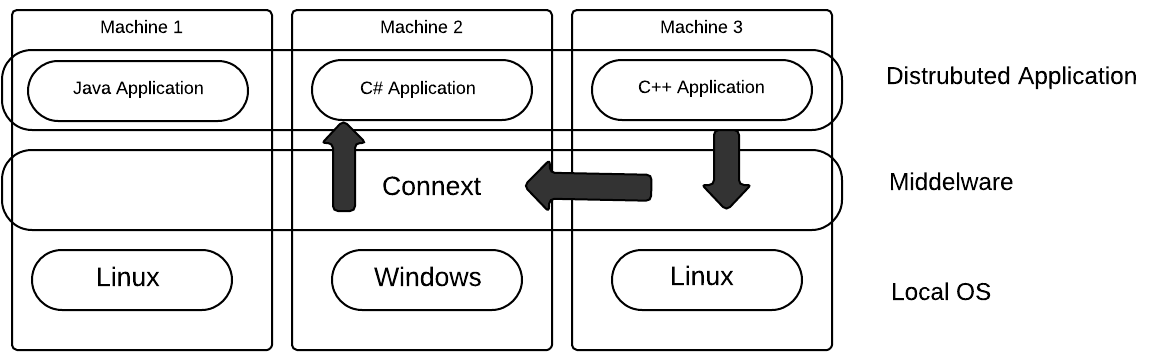
\includegraphics[scale=0.35]{MiddelwareImplementation}
		\end{figure}
				
	\end{frame}
		
	
\section{What is IDL}
	\begin{frame}
		\frametitle{What is IDL (Interface Description Language)?}
		
		\begin{itemize}
		\item Cross-platform interface
		\item Object Management Group (OMG)
		\item Topics can be published and subscribed with IDL
		
		\end{itemize}
		
	\end{frame}
	
	
	
\section{DDS components}
	\begin{frame}
		\frametitle{DDS components}
		
	
		\begin{itemize}
		\item Data Local Reconstruction Layer (DLRL)
		
			\begin{itemize}
			\item App level -- Global Class
			\item Not supported any more
			\end{itemize}
		
		\item Data Centric Publish Subscribe (DCPS)
		
			\begin{itemize}
			\item Exchange of data between app-layer and hardware
			\end{itemize}
		
		\end{itemize}
		
	\end{frame}
	
	
	
\subsection{Publish/Subscriber with DDS}
	\begin{frame}
		\frametitle{Publish/Subscriber with DDS}

		\begin{figure}[hbtp]
		\centering
		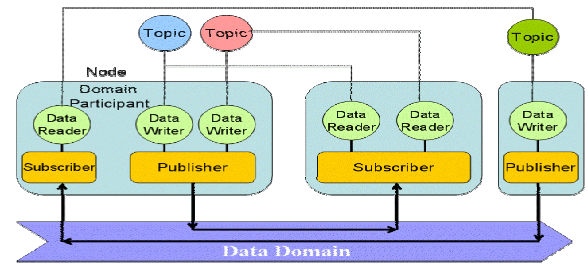
\includegraphics[scale=0.65]{DDSentities}
		\end{figure}
	\end{frame}

	
\section{Space, time, and flow decoupling}
	\begin{frame}
		\frametitle{What does space, time, and flow decoupling mean?}
		
		\begin{itemize}
		\item Space -- Publish and subscribers
		\item Time -- Asynchronous 
		\item Flow -- No blocking of flow
		
			\begin{itemize}
			\item Queues stores the published data
			\end{itemize}
			
		\item RTI does all the above
						
		\end{itemize}
		
	\end{frame}
	
	
\section{The role of quality of service}
	\begin{frame}
		\frametitle{What is the role of quality of service (QoS) parameters?}
		
		\begin{itemize}
		\item Filter data from DataWriters
		\item Filter data on Publishers and Subscribers
		\item Filter data to DataReaders
		\item Changeable in an \code{.xml}-file
		\end{itemize}
		
	\end{frame} 
 	
	
\section{DDS example}
	\begin{frame}
		\frametitle{Prototype of DDS}
		
		\begin{figure}[hbtp]
		\centering
		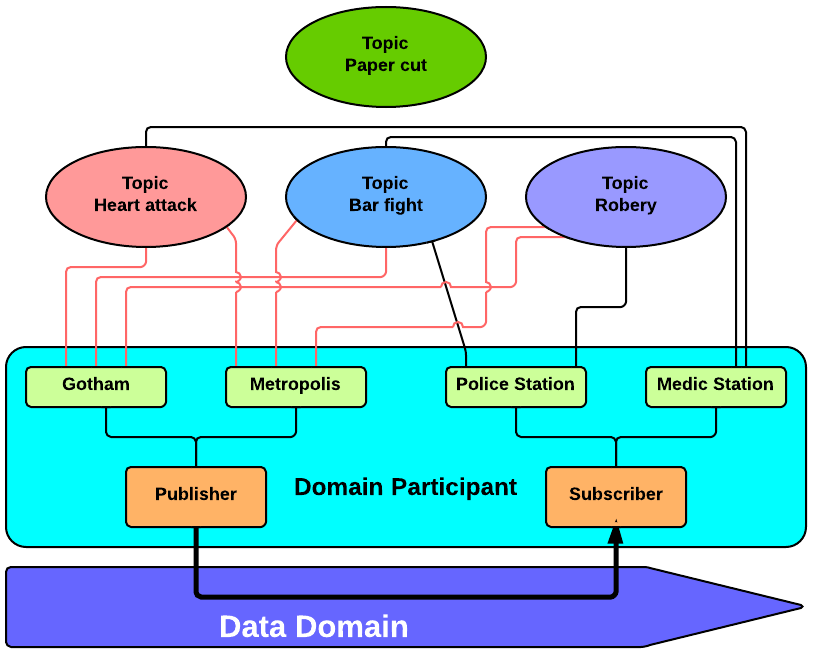
\includegraphics[scale=0.33]{Prototype}
		\end{figure}
		
	\end{frame} 
\end{document}